\documentclass{article}

\usepackage{tikz}
\usetikzlibrary{calc}

\begin{document}
	\begin{center}
		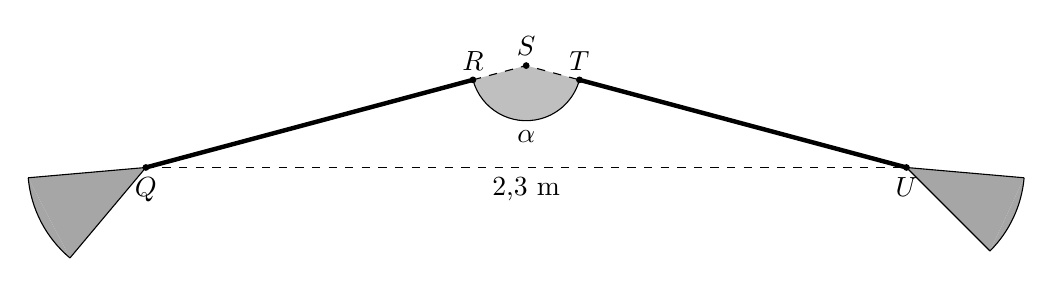
\begin{tikzpicture}
			\coordinate (S) at (0,0);
			\coordinate (T) at (-15:0.7);
			\coordinate (R) at (195:0.7);
			\coordinate (U) at (-15:5);
			\coordinate (Q) at (195:5);
			
			%desenhando a pá da direita
			\coordinate (U1) at ($(U) + (-5:1.5)$);
			\coordinate (U2) at ($(U) + (-45:1.5)$);
			\draw[fill=gray!70] (U1) -- (U) -- (U2);
			\draw[fill=gray!70] (U1) arc (-5:-45:1.5); 
						
			%desenhando a pá da esquerda
			\coordinate (Q1) at ($(Q) + (185:1.5)$);
			\coordinate (Q2) at ($(Q) + (230:1.5)$);
			\draw[fill=gray!70] (Q1) -- (Q) -- (Q2);
			\draw[fill=gray!70] (Q1) arc (185:230:1.5);
			
			%desenhando arco no centro
			\draw[fill=gray!50, dashed] (R) -- (S) -- (T);
			\draw[fill=gray!50] (R) arc (-165:-15:0.7);
			
			%desenhando segmentos
			\draw [dashed] (Q) -- (U);
			\draw [ultra thick] (T) -- (U);
			\draw [ultra thick] (R) -- (Q);
			
			%marcando os pontos
			\draw[fill=black] (Q) circle(1pt) node[below]{\(Q\)};
			\draw[fill=black] (R) circle(1pt) node[above]{\(R\)};
			\draw[fill=black] (S) circle(1pt) node[above]{\(S\)};
			\draw[fill=black] (T) circle(1pt) node[above]{\(T\)};
			\draw[fill=black] (U) circle(1pt) node[below]{\(U\)};
			
			%marcando labels
			\draw (-90:0.7) node[below]{\(\alpha\)};
			\draw (-90:1.3) node[below]{2,3 m};
		\end{tikzpicture}
	\end{center}
\end{document}